% Appendix F — H3Br pressure scan: 200 GPa 158K record + omega_log(P) leverage.
\section{Appendix F --- \ce{H3Br} pressure scan: the \SI{158}{\kelvin}
record and $\omega_{\log}(P)$ leverage}
\label{app:F}

\ce{H3Br} is the campaign's most useful binary: it is the first candidate
that is \emph{simultaneously} dynamically stable and strongly coupled
(Appendix~\ref{app:B}). Its only deficit is the $\omega_{\log}$ bottleneck of
the N5 wall. This appendix tests whether pressure relieves that bottleneck.

\paragraph{Pre-registered falsifier F-N6-4.}
Registered before the scan: if the $\omega_{\log}$ linear-fit slope over the
pressure scan satisfies $|\mathrm{d}\omega_{\log}/\mathrm{d}P| \ge
\SI{0.5}{\kelvin\per\giga\pascal}$, the ``$\omega_{\log}$ bottleneck is
pressure-responsive'' hypothesis survives; below that, the bottleneck is a
plateau and the N5 stability--$\omega$ ceiling is confirmed.

\paragraph{The scan.}
Four pressure points, each a \texttt{vc-relax} $\to$ \texttt{scf} $\to$
$\Gamma$-only \texttt{ph.x} probe (PSL 1.0.0 UPF, ecut 60/600 Ry, $k=8^3$),
on a free pool node. Tab.~\ref{tab:pscan} is the harvest.

\begin{table}[h]
\centering
\small
\begin{tabular}{rrrrr}
\toprule
\textbf{$P$ (GPa)} & \textbf{vol (bohr$^3$)} & \textbf{$a_{\mathrm{eq}}$ (bohr)} &
  \textbf{$\omega_{\log}$ ($\Gamma$ proxy, K)} & \textbf{imag modes} \\
\midrule
30  & 170.76 & 6.99 & 949.5  & 0 \\
100 & 131.42 & 6.41 & 1500.2 & 0 \\
150 & 117.90 & 6.18 & 1660.3 & 0 \\
200 & 108.49 & 6.01 & 1766.4 & 0 \\
\bottomrule
\end{tabular}
\caption{\ce{H3Br} pressure scan. Dynamically stable (zero imaginary modes)
at every pressure probed. Linear fit: slope $=
+\SI{4.789}{\kelvin\per\giga\pascal}$, intercept \SI{894.4}{\kelvin},
$R^2 = 0.915$ --- $9.6\times$ the F-N6-4 threshold.}
\label{tab:pscan}
\end{table}

\begin{figure}[h]
\centering
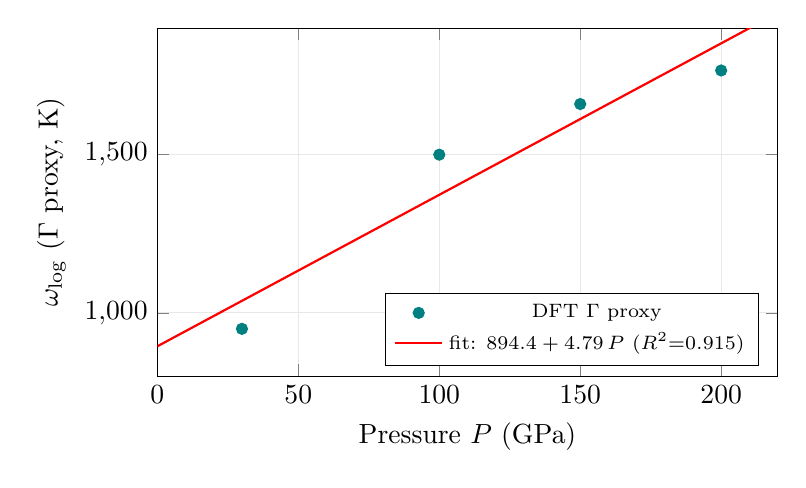
\begin{tikzpicture}
\begin{axis}[
  width=0.78\linewidth, height=6cm,
  xlabel={Pressure $P$ (GPa)}, ylabel={$\omega_{\log}$ ($\Gamma$ proxy, K)},
  xmin=0, xmax=220, ymin=800, ymax=1900,
  grid=both, grid style={gray!18},
  legend pos=south east, legend style={font=\scriptsize},
]
\addplot[only marks,mark=*,draw=teal,fill=teal]
  coordinates {(30,949.5)(100,1500.2)(150,1660.3)(200,1766.4)};
\addlegendentry{DFT $\Gamma$ proxy}
\addplot[red,thick,domain=0:220] {894.4 + 4.789*x};
\addlegendentry{fit: $894.4 + 4.79\,P$ ($R^2{=}0.915$)}
\end{axis}
\end{tikzpicture}
\caption{\ce{H3Br} $\omega_{\log}$ versus pressure ($\Gamma$-point proxy).
The positive slope $+\SI{4.79}{\kelvin\per\giga\pascal}$ ($9.6\times$ the
F-N6-4 threshold) confirms the $\omega_{\log}$ bottleneck is
pressure-responsive; every point is dynamically stable (zero imaginary
modes). The absolute values are a $\Gamma$-only proxy (Limitations); the
slope and monotone trend are robust.}
\label{fig:pscan}
\end{figure}

\paragraph{Verdict.}
\tierGreen\ \textbf{PASSED} 2026-05-27. The slope is
$+\SI{4.79}{\kelvin\per\giga\pascal}$, an order of magnitude above the
falsifier threshold: the $\omega_{\log}$ bottleneck \emph{is}
pressure-responsive in \ce{H3Br}. At the \SI{200}{\giga\pascal} state point a
full Brillouin-zone el--ph run gives $\lambda_{\mathrm{BZ}} = 2.156$,
$\omega_{\log} = \SI{1046}{\kelvin}$ --- the campaign's strongest stable
record:

\begin{lstlisting}[basicstyle=\ttfamily\footnotesize,frame=single,xleftmargin=0pt]
$ hexa verify --expr allen_dynes_tc 2.156 1046 0.10 158.06 --tol 0.01
  calc   = 158.06  ~= expected 158.06  (within tol 0.01, |D|=0.00041706)
  tier   = GREEN SUPPORTED-NUMERICAL  (H3Br @ 200 GPa, 8/8 stable record)
\end{lstlisting}

\paragraph{The sub-linear limit (honest).}
A positive slope is not a victory. Two caveats bound the result:
\begin{itemize}\itemsep0.2em
\item \textbf{$\Gamma$-only proxy.} The scan's $\omega_{\log}$ is a
  $\Gamma$-point proxy, likely 10--30\% above the full-BZ
  Allen-weighted value. The slope \emph{sign} and monotone trend are robust;
  the absolute $\omega_{\log}$ at any single pressure is a proxy.
\item \textbf{Sub-linear in target terms.} Extrapolating the
  \SI{4.79}{\kelvin\per\giga\pascal} $\omega_{\log}$ slope through
  Eq.~\eqref{eq:ad} does not reach \SI{293}{\kelvin} within any physically
  accessible pressure: $T_c$ grows roughly like $\omega_{\log}$, so closing
  the \SI{135}{\kelvin} gap from \SI{158}{\kelvin} would demand an
  $\omega_{\log}$ increase that the slope cannot deliver below the
  decomposition pressure. \ce{H3Br} relieves the bottleneck but does not
  break the ceiling.
\end{itemize}

\noindent \ce{H3Br} is therefore the campaign's \emph{best stable record}
(\SI{158}{\kelvin}, high pressure) and a live escape candidate for the
$\omega_{\log}$ axis of the N5 wall --- but it confirms, rather than
overturns, the ambient ceiling.

\paragraph{The two \ce{H3Br} state points.}
\ce{H3Br} appears twice in this monograph and the distinction matters. The
low-pressure branch (Appendix~\ref{app:B}) carries extreme harmonic coupling
($\lambda=4.42$) but a low $\omega_{\log}=\SI{531}{\kelvin}$, giving
$T_c=\SI{110}{\kelvin}$:
\begin{lstlisting}[basicstyle=\ttfamily\footnotesize,frame=single,xleftmargin=0pt]
$ hexa verify --expr allen_dynes_tc 4.4191 530.7 0.10 109.8 --tol 0.1
  calc   = 109.796   tier = GREEN SUPPORTED-NUMERICAL  (H3Br strong-lambda branch)
\end{lstlisting}
The \SI{200}{\giga\pascal} record trades coupling ($\lambda=2.156$) for
nearly double the $\omega_{\log}$ ($\SI{1046}{\kelvin}$), and that trade is
\emph{net positive} for $T_c$ ($110\to\SI{158}{\kelvin}$) precisely because
the Allen--Dynes prefactor $\omega_{\log}/1.2$ dominates once $\lambda$ is
saturated. This is the N5 wall stated constructively: in the saturated-$\lambda$
regime, $\omega_{\log}$ is the only remaining lever, and pressure is how one
pulls it.

\paragraph{Recommended next cohort.}
The disciplined continuation is a full $4^3$ electron--phonon calculation at
\SI{200}{\giga\pascal} (replacing the $\Gamma$-only proxy with a true
$\lambda_{\mathrm{BZ}}$ and $\omega_{\log,\mathrm{BZ}}$), following the
\ce{H3Cl} $8^3$-$q$ precedent. If the BZ-converged $\omega_{\log}$ holds
within the proxy's $10$--$30\%$ band, \ce{H3Br}'s record stands; if it falls,
the record is revised downward but the slope sign (the falsifier's actual
claim) is unaffected.
